\section{Постановка эксперимента}

\subsection{Конфигурация экспериментального стенда}

\subsubsection{Аппаратное обеспечение}

Процессоры 2 x Intel Xeon Platinum 8168 CPU @ 2.7 GHz.
Технология Hyper-Threading отключена для уменьшения нежелательного влияния на время обслуживания заявок в системе \cite{LowLatencyHT}.

Оперативная память: DDR4-2666 128 GiB.

\subsubsection{Программное обеспечение}

Операционная система Red Hat Enterprise Linux Server release 7.8 (Maipo).
Ядро Linux 3.10.0-1127.el7.x86\_64

Компилятор C++ Clang 6.0.1.

Стандартная библиотека C++: libstdc++ 8.1.0.

Библиотека Boost.Interprocess 1.68.0.

\subsection{Конфигурация экспериментальной системы}

Система для проведения эксперимента состоит из двух процессов:
\begin{itemize}
\item Процесс-шлюз отвечает за преобразование заявок из формата внешнего мира во внутренний формат системы и обратно. 
\item Процесс-обработчик совершает некоторые преобразования над заявкой и отправляет результат за пределы системы через процесс-шлюз.
\end{itemize}

Процессы выполняются на двух процессорах, расположенных в разных разъемах на материнской плате физического узла.

Снаружи системы находится симулятор внешнего мира. Он генерирует поток заявок в систему и получает результат обработки заявки в системе. Схема взаимодействия процессов в эксперименте представлена на Рисунке \ref{chapter41:SystemSchema}.

\begin{figure}[!h]
\caption{Схема взаимодействия процессов в эксперименте}
\label{chapter41:SystemSchema}
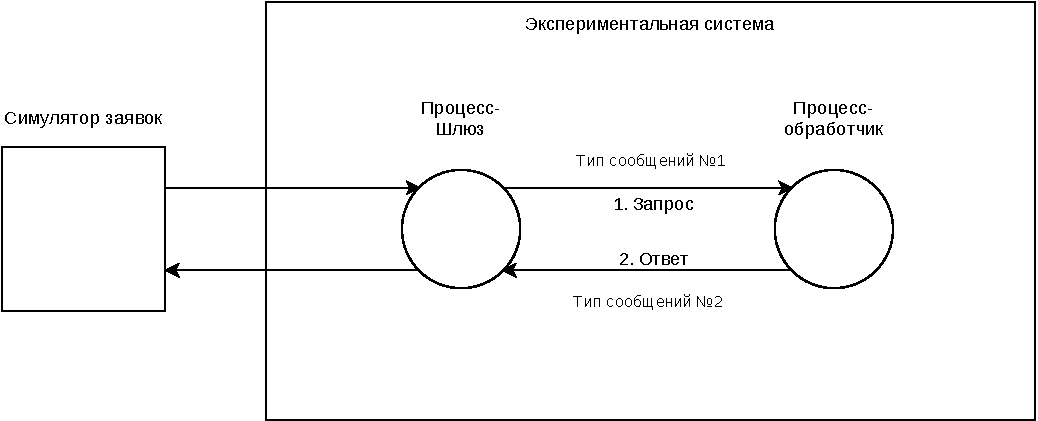
\includegraphics[width=\textwidth]{../../graphics/schemes/SystemSchema}
\end{figure}

В настоящей работе замеряется временная задержка на передачу данных между процессами внутри системы, а именно из процесса-шлюза в процесс-обработчик и обратно (сообщения типа №1 и №2 в запросе и ответе между процессом-шлюзом и процессом обработчиком на Рисунке \ref{chapter41:SystemSchema}).

Процессы системы взаимодействуют используют одно соединение, в рамках которого заявки обрабатываются строго последовательно.
Обслуживание включает в себя: прием заявки, выполнение пользовательской логики над заявкой и, если необходимо, отправка ответа.
Временной задержкой на передачу данных в настоящей работе принимается временной промежуток от начала отправки заявки до \textbf{начала обработки заявки}. Таким образом, возможен случай, когда во время обработки очередной заявки процессом в очереди уже находится следующая заявка, временная задержка на передачу которой, таким образом, увеличится на время обработки текущей заявки.

Данный сценарий актуален для процесса-обработчика, в котором обслуживание заявки осуществляется непосредственно в транспортном потоке
В случае с процессом-шлюзом транспортный поток только читает и диспетчеризует асинхронную обработку заявки, т.е. не выполняет обработку самой заявки.

% \textbf{TBD: надо как- то адекватно это описать}
Пользовательская логика процесс-обработчика в среднем отклоняет 25\% заявок, в то время как 75\% заявок отправляются в процесс-шлюз.

\subsection{Используемые обозначения}

Все величины с, указанные с интервалом, указаны с 95\% доверительной вероятностью.

\begin{itemize}
\item $\Delta$ -- временная задержка между сериями заявок;
\item $\delta$ -- временная задержка между заявками в серии;
\item транспортный поток -- поток из пула транспортных потоков, непосредственно обслуживающий получаемые заявки.
\end{itemize}

\subsection{Характер экспериментальной нагрузки}

Симулятор отправляет в систему заявки сериями с интервалом $\Delta$ в \textit{~10 мс} по \textit{4} заявки в серии с интервалом $\delta$ \textit{~60 мкс} между ними. Так как для каждого эксперимента производился отдельный запуск симулятора, средние значения обозначенных величин приведены для каждого эксперимента отдельно.

\subsection{Время обслуживания заявок в процессах}
% \textbf{TBD: разобраться с обработкой соединений и обслуживанием заявок. Должно быть одно слово для обозначения одной сущности.}

На Рисунке \ref{chapter41:EngineLatency} представлена гистограмма времени обслуживания заявок в процессе-обработчике. Время обслуживания заявок с 95\% доверительной вероятностью укладывается в диапазон \textit{13 $\pm$ 7 мкс}.
\begin{figure}[!h]
\caption{Гистограмма времени обслуживания заявки в процессе-обработчике}
\label{chapter41:EngineLatency}
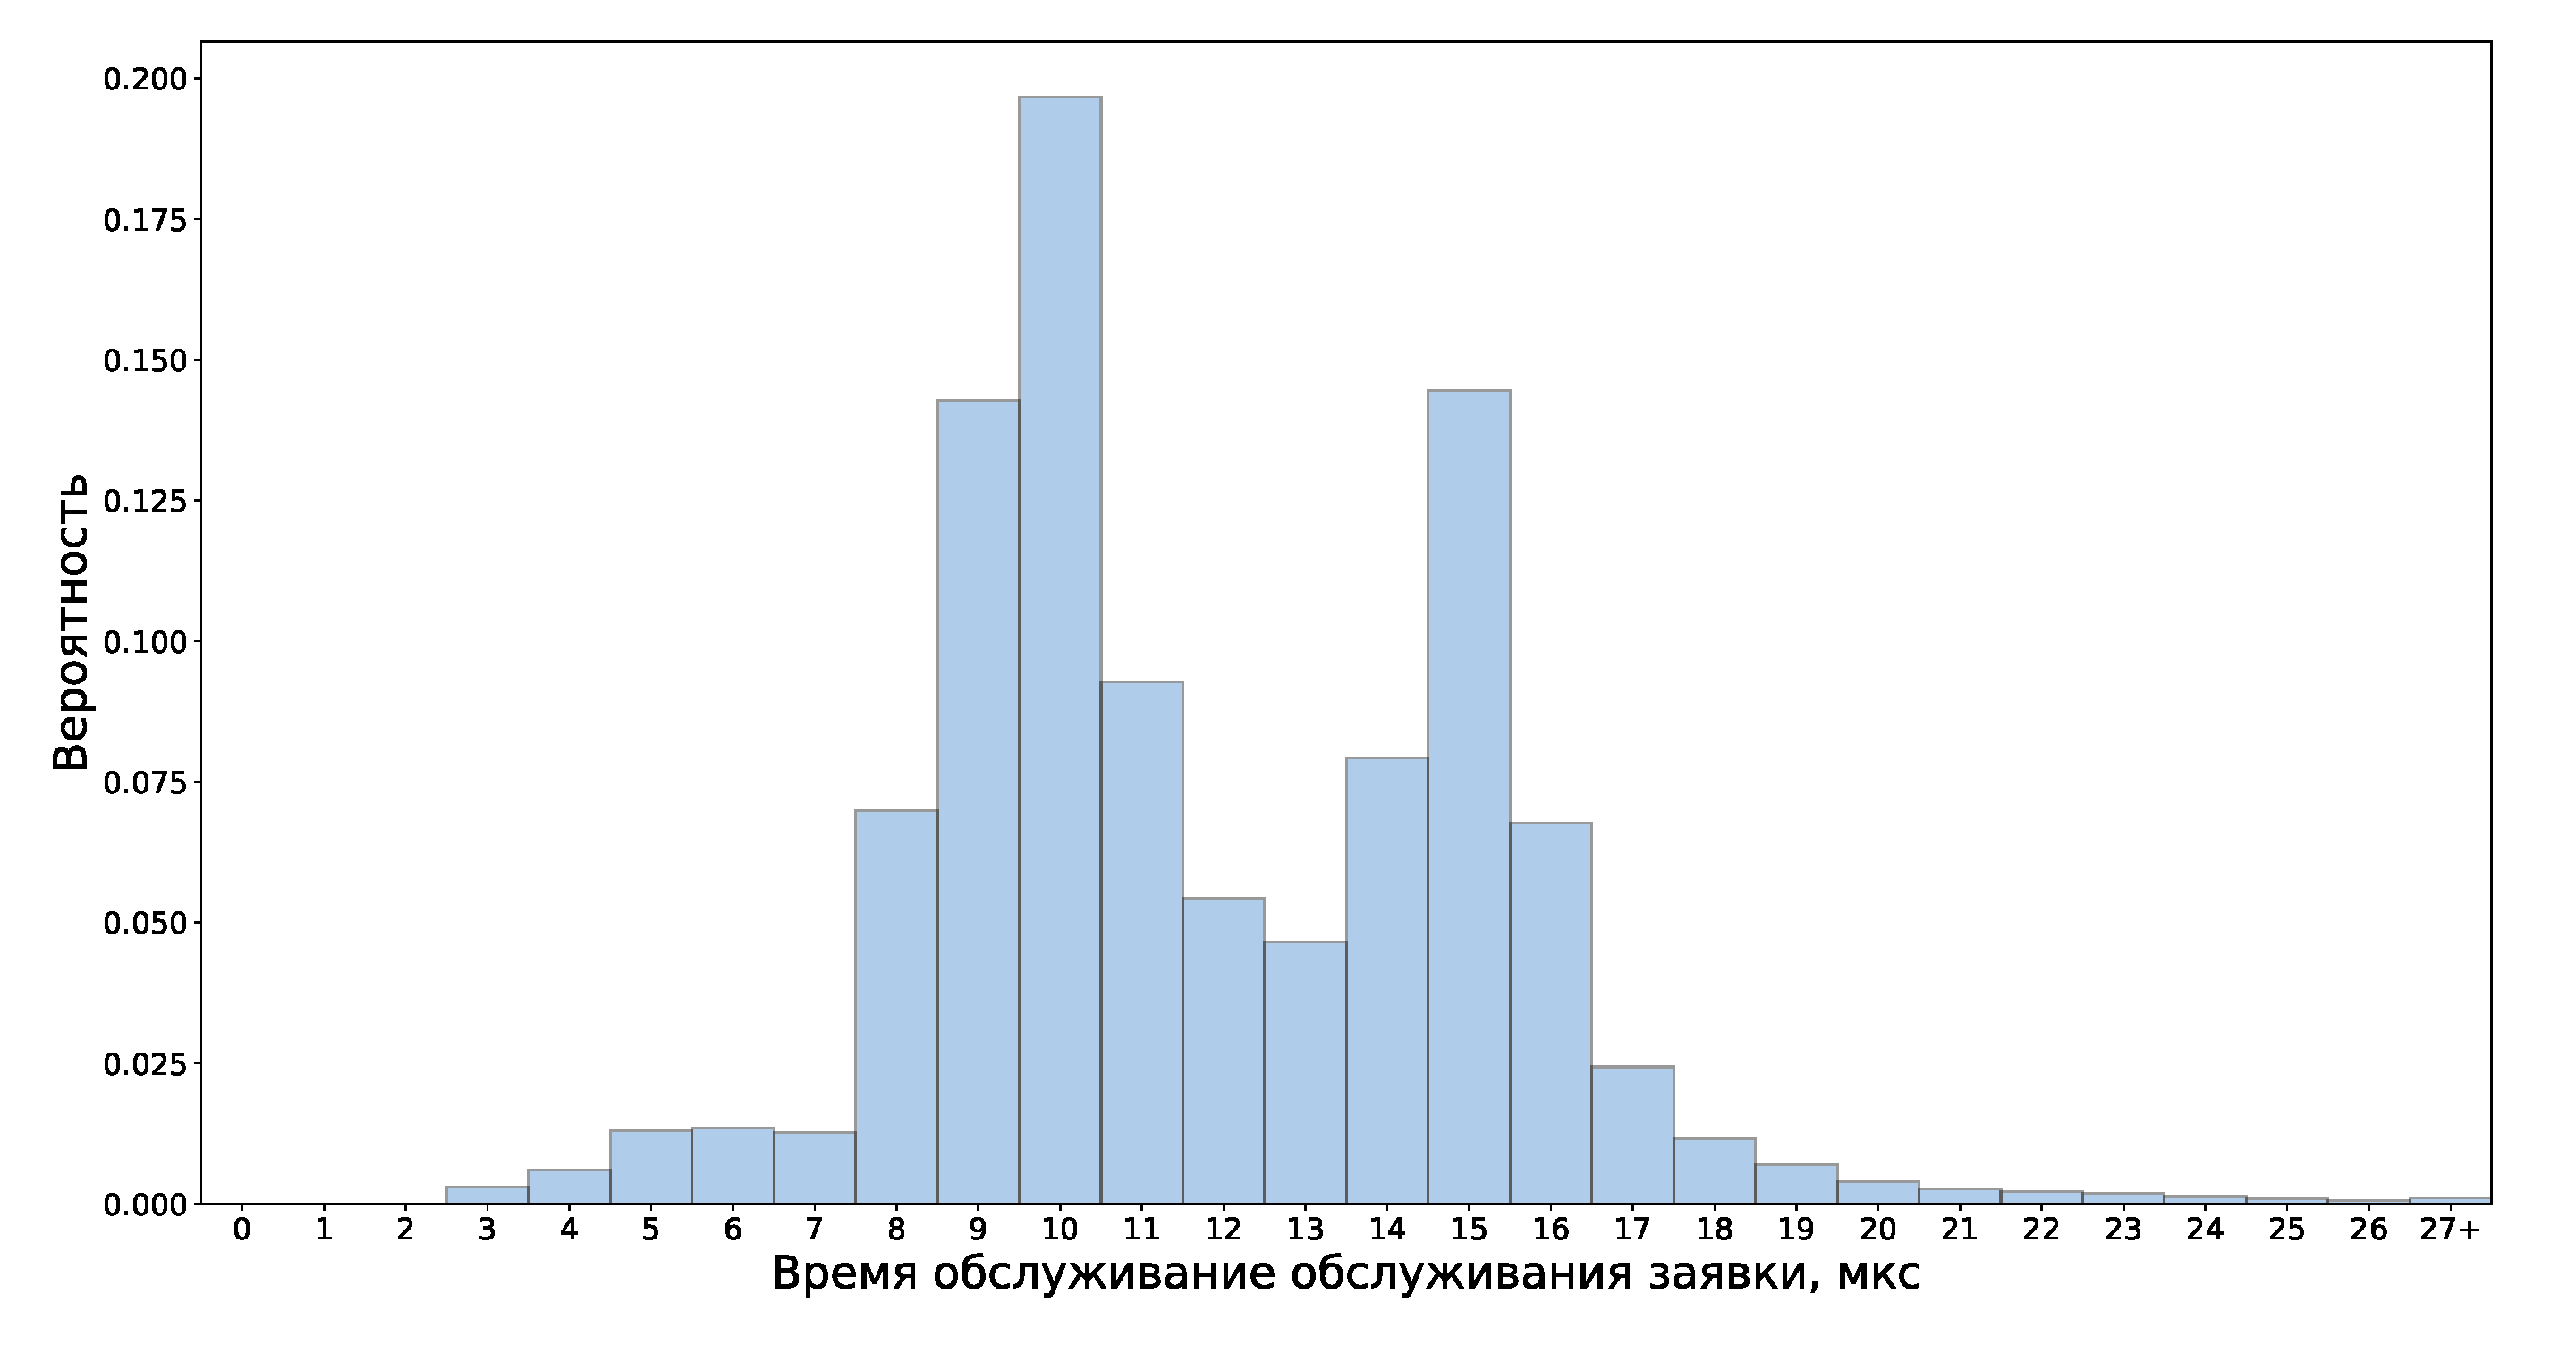
\includegraphics[width=\textwidth]{../../graphics/hist/Engine}
\end{figure}

На Рисунке \ref{chapter41:TRLatency} представлена гистограмма времени обслуживания заявок в процессе-шлюзе. Время обслуживания заявок с 95\% доверительной вероятностью укладывается в диапазон \textit{19 $\pm$ 6 мкс}.
\begin{figure}[!h]
\caption{Гистограмма времени обслуживания заявки в процессе-шлюзе}
\label{chapter41:TRLatency}
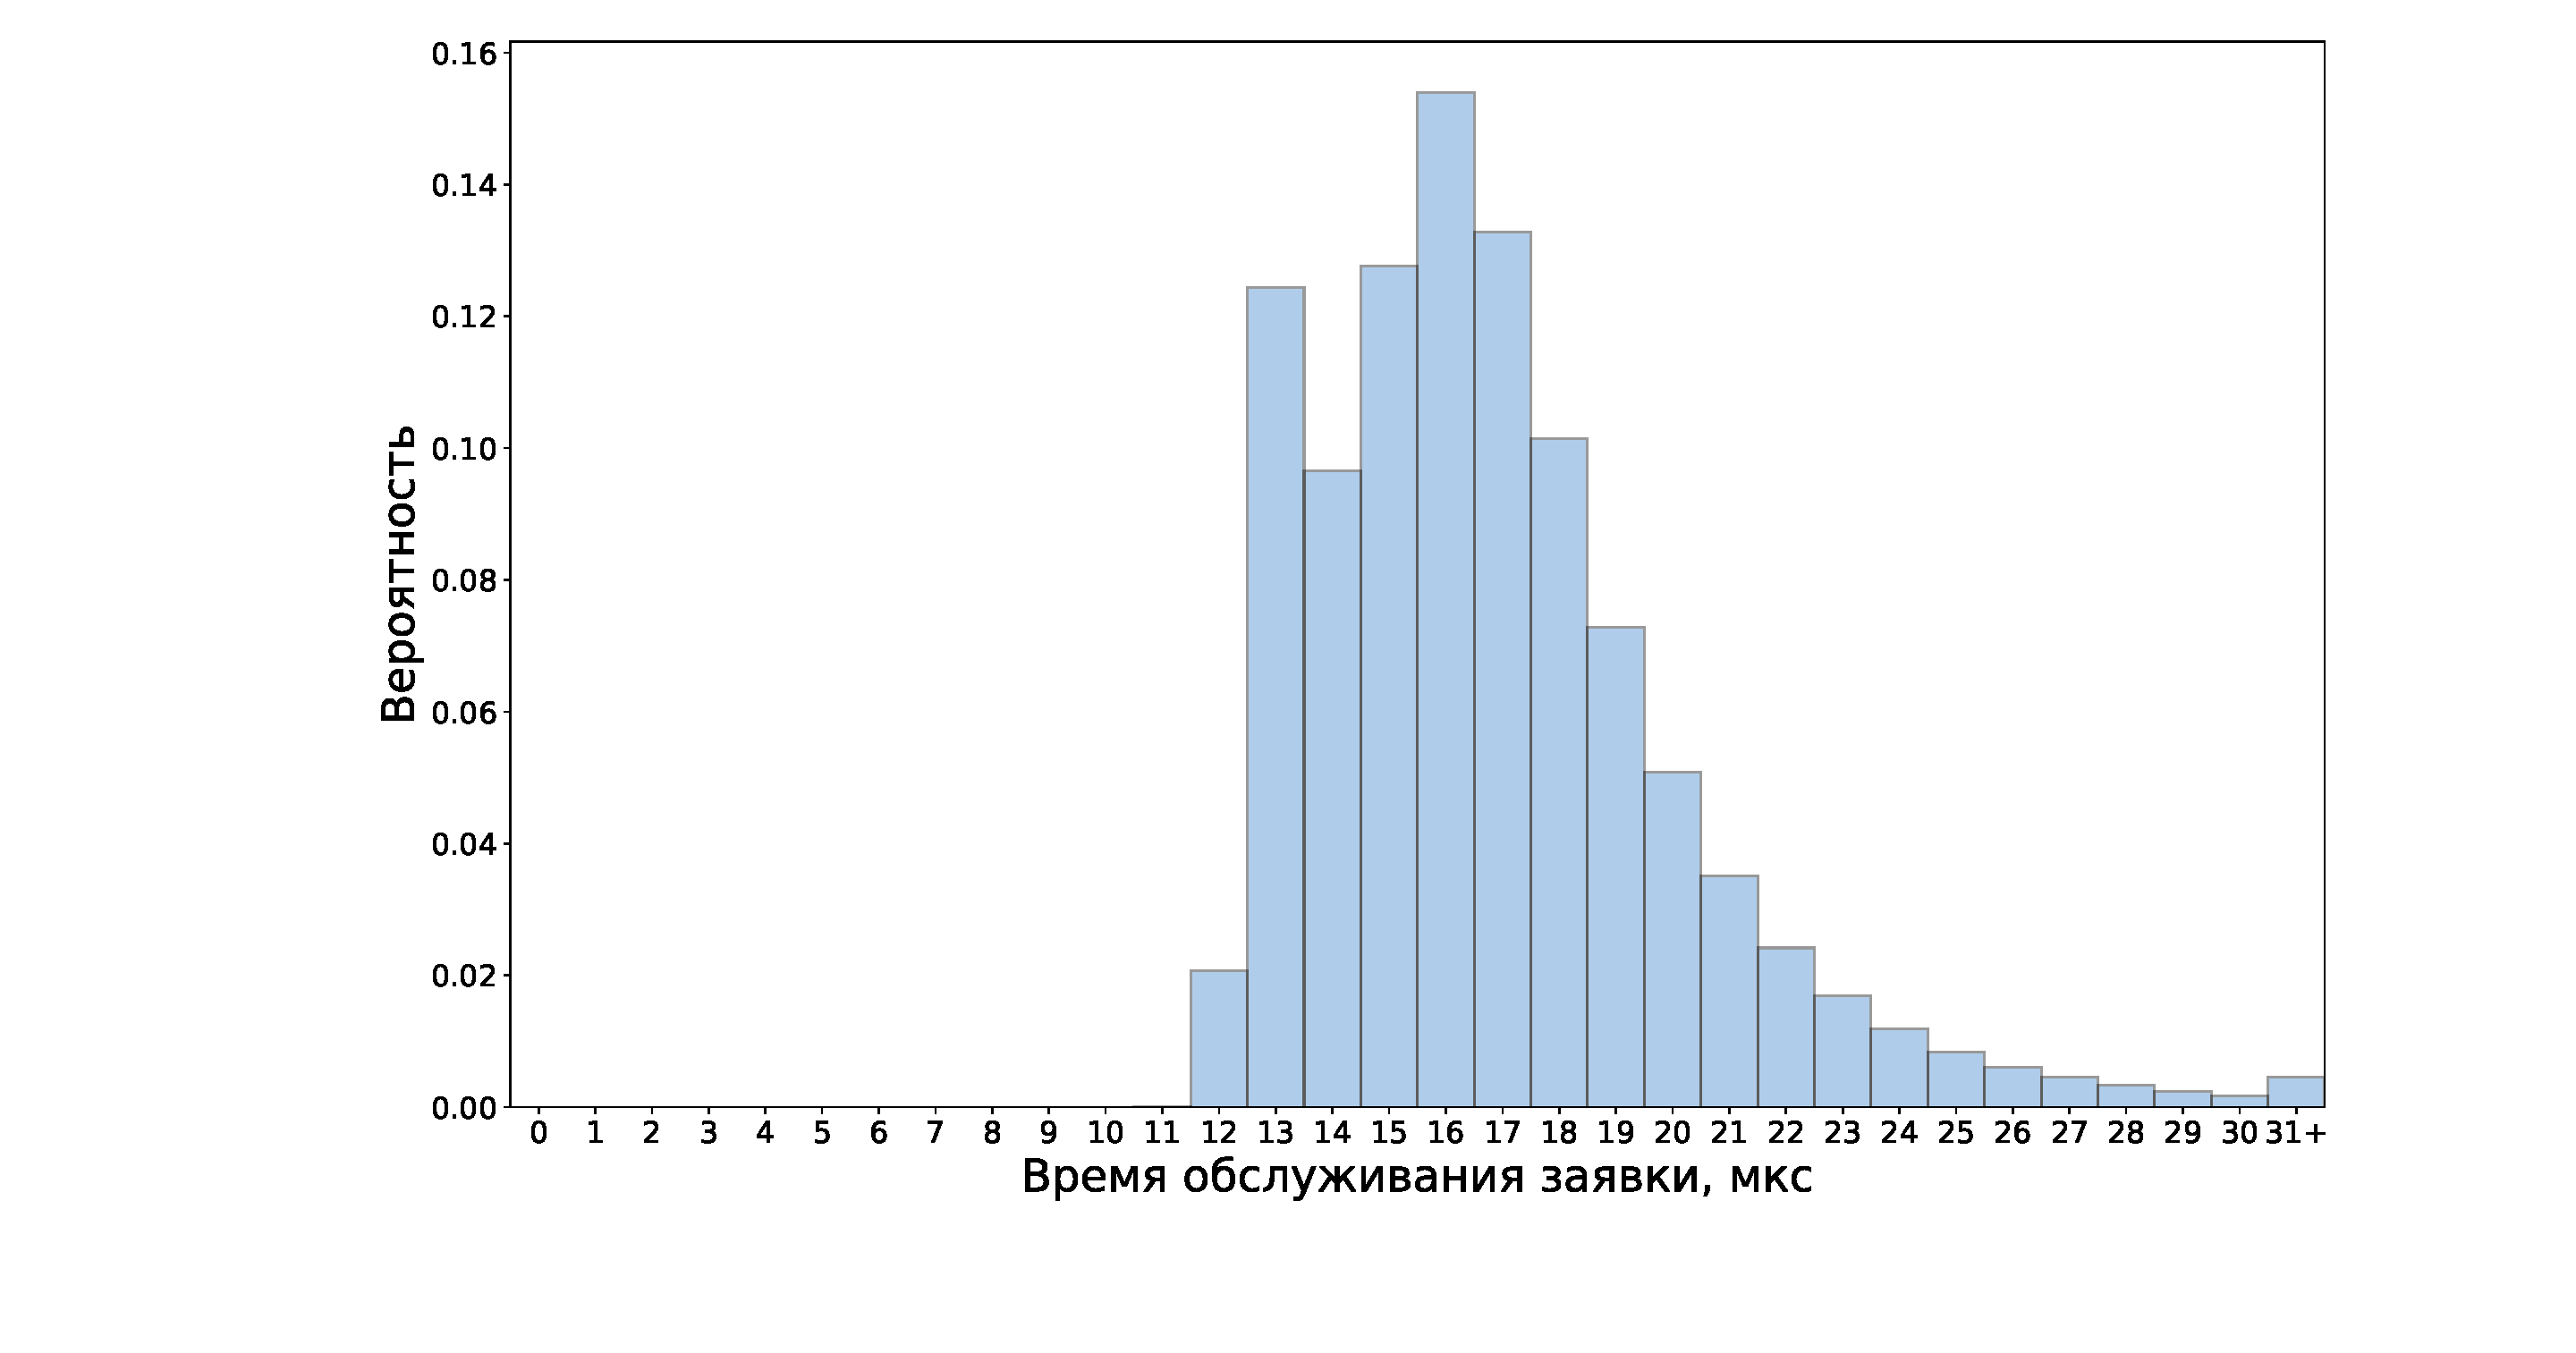
\includegraphics[width=\textwidth]{../../graphics/hist/TR}
\end{figure}

% \textbf{TBD: а надо ли мне вообще говорить тогда про время обслуживания заявок в процессе-шлюзе? Может, убрать совсем?}
Как было сказано выше, в процессе-шлюзе заявки обслуживания вне транспортного потока, поэтому время обслуживания заявок в процессе-шлюзе не влияет на временную задержку на передачу данных. В случае с процессом-обработчиком значительная часть обслуживания заявки выполняется именно в транспортном потоке, что влияет на временную задержку на передачу данных, т.к. нахождение в очереди влияет на данный показатель.
